\documentclass[Space3_Assign1.tex]{subfiles}

\begin{document}
\newpage
\section{Simulating Perturbations}

\subsection{Introduction}
The basic keperian model only accounted for an ideal two body system with no other effects when in reality, other forces act of the satellite. Compared to the gravitational motion between the Earth and the satellite however, these other effects are small. Therefore, they can be mathematically modelled as perturbations. While it is still an approximation, the error is reduced. Types of perturbations include;
\begin{itemize}
\item gravitational effects: such as the oblate Earth, third-body interactions such as the Moon, Sun or other planets
\item drag forces: from the Earth's atmosphere and from solar radiation pressure
\item unexpected thrusting: from malfunctioning thrusters
\end{itemize} 


\subsubsection{Earth oblateness}
For the standard simulation model in Question 1, it was assumed that the Earth was spherical. A perfectly spherical mass has an inverse square relation of the gravitational field to the force applied on a body. However, the Earth is slightly oblate, as it is flatter at the poles and wider at the equator than a sphere. 

Unlike using the keplerin model of Question 1, the classical orbital parameters change through time.

\subsubsection{Van Allen Probes}
Due to the highly elliptical orbit of the Van Allen Probes, most of the time the satellite is in MEO away from the Earth's atmosphere. As the inclination of the orbit keeps the satellite close to the equator, the perturbation due to the non-spherical earth 

Newtown's second law and his law of gravitation results in the following equation in the ECI frame [1].
\begin{eqnarray}
\av{r}+\frac{\mu\dv{r}}{r^3} = a\frac{3J_2\mu R_e^2}{2R^5}\left( \left( 5\frac{z^2}{R^2}-1 \right)(x\hat{i}+y\hat{j}) + z\left( 5\frac{z^2}{R^2}-3 \right)\hat{k} \right) 
\end{eqnarray}

\subsection{Methodology}
Equinoctial elements were used to remove the possible singularities that affect classical elements. The 



\subsection{Results/Discussion}
For the perturbation model the calculated orbital period was 8.4722 hours, compared to the 8.9518 hrs of the keperlian model. This is because the satellite is pulled further around the Earth as it crosses the equator. 

\begin{figure}[h!]
\centering
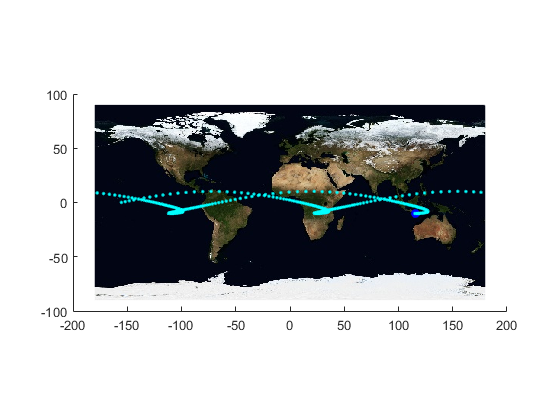
\includegraphics[width=1\linewidth]{Q2_gnd}
\caption{Ground trace of perturbation model}
\label{fig:Q2_gnd}
\end{figure}

The J2 perturbation model was implemented for the satellite Van Allen Probe A and integrated over twelve days and compared to the TLEs in the same time frame. Figure \ref{fig:Q2classical_overtime} shows the progression of the classical elements. The right ascending node and argument of perigee agreed very well with the perturbation model, indicating that the oblate Earth effect is strong on the satellite. The general trends of the inclination, semi-major axis and eccentricity indicate that there is another effect occurring on the satellite, such as atmospheric drag effects as it has a very low perigee. However, the percentage of the change in the parameter is very small < 0.1 \%. Figure \ref{fig:Q2equinoctial_overtime} displays the equinoctial elements, with strong agreement for all parameters except for the semilatus rectum (p) however it is again <0.6 \% difference and exists for the same reasons as prior. The parameter $\theta$ was calculated from the TLEs using the revolution number plus the calculated true anomaly from eq\eqref{trueanom}. \\\indent
In the keplerian model, the classical elements are not variables, but are constants used the in the equations for position and velocity in the perifocal frame. The blue circle marker on Figure \ref{fig:Q2classical_overtime} shows the Keplerian value, and the initial value used in the perturbation model.




\begin{figure}[h!]
\centering
\caption{Classical Elements over 12 days}
\label{fig:Q2classical_overtime}
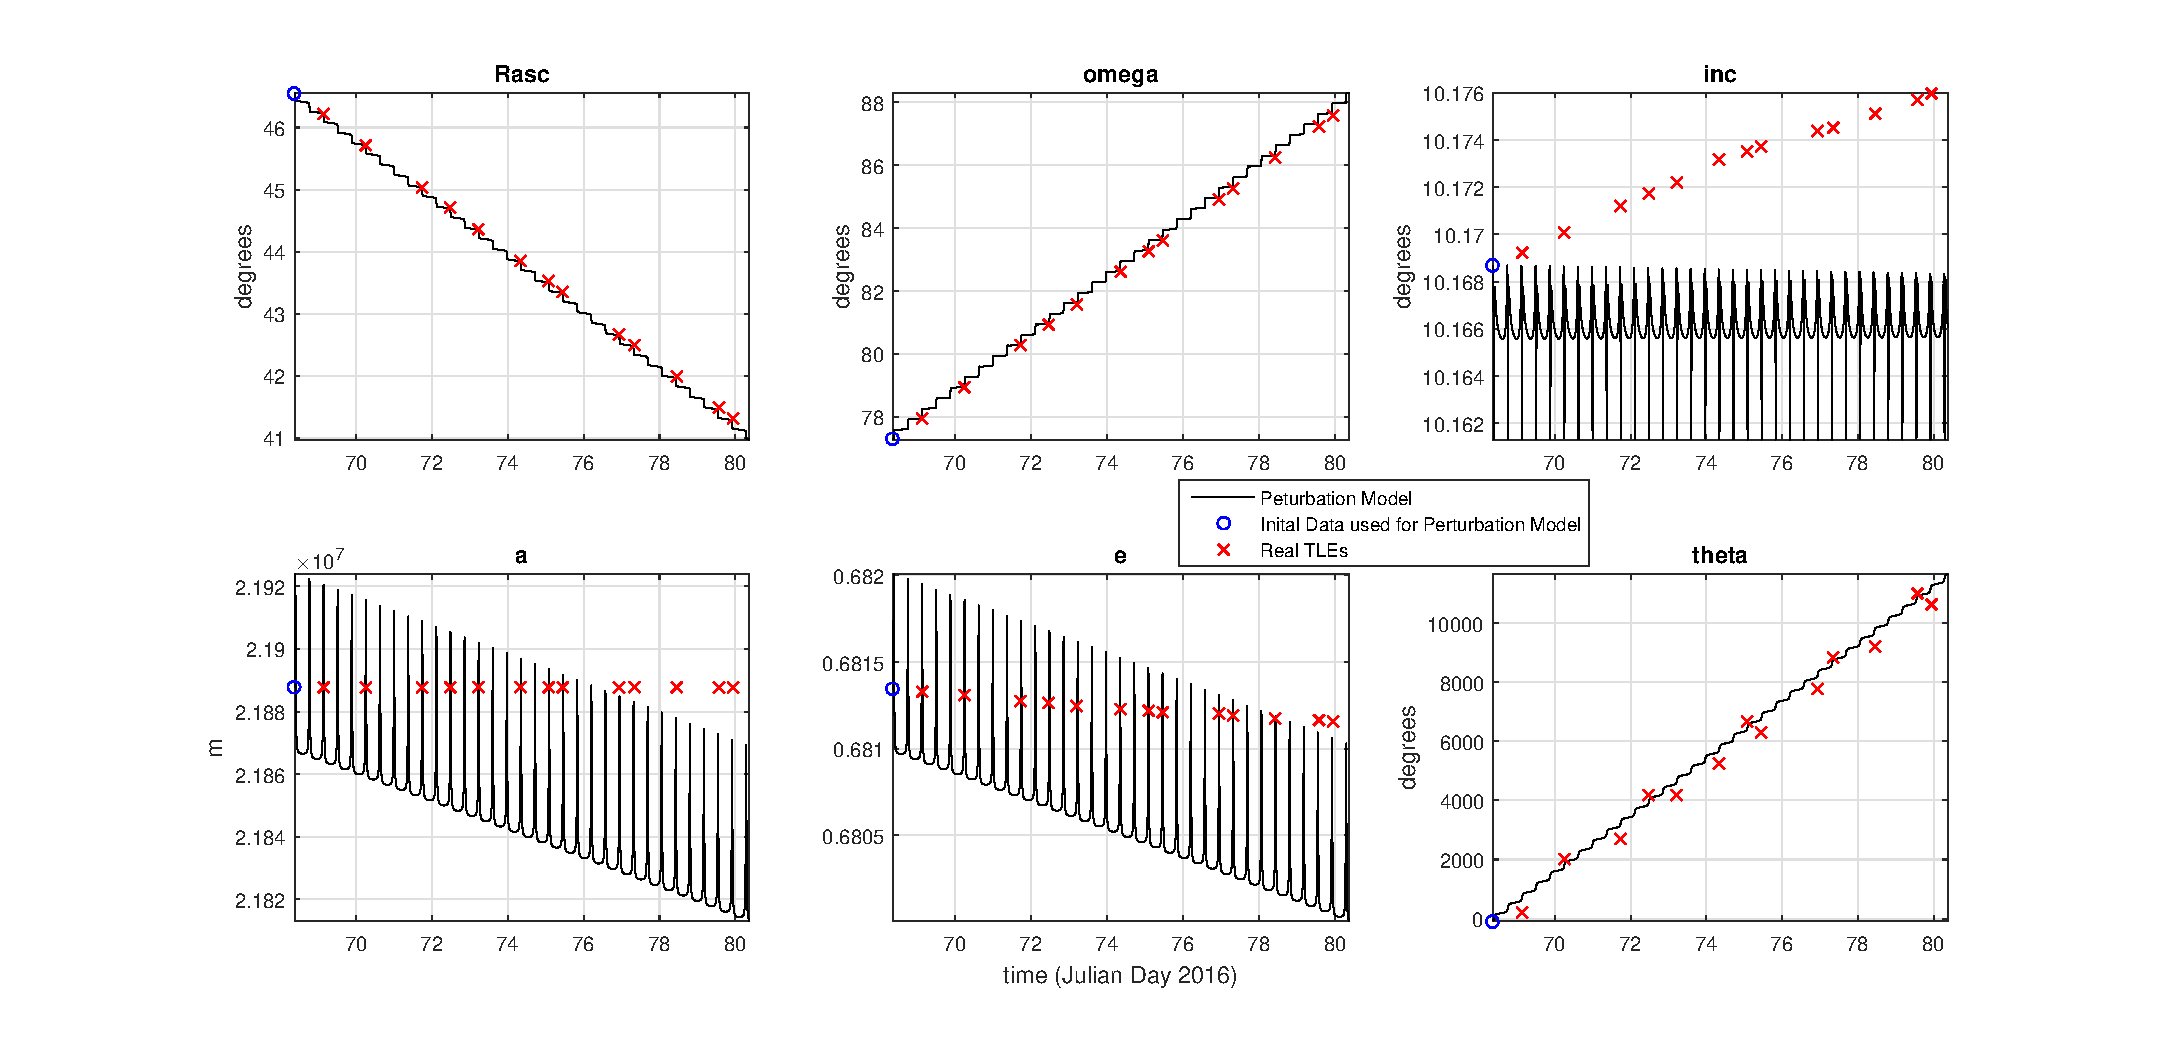
\includegraphics[trim = {3cm 0 3cm 0},clip,width=1\linewidth]{Q2classical_overtime.eps}
\end{figure}
\begin{figure}[h!]
\centering
\caption{Equinoctial Elements over 12 days}
\label{fig:Q2equinoctial_overtime}
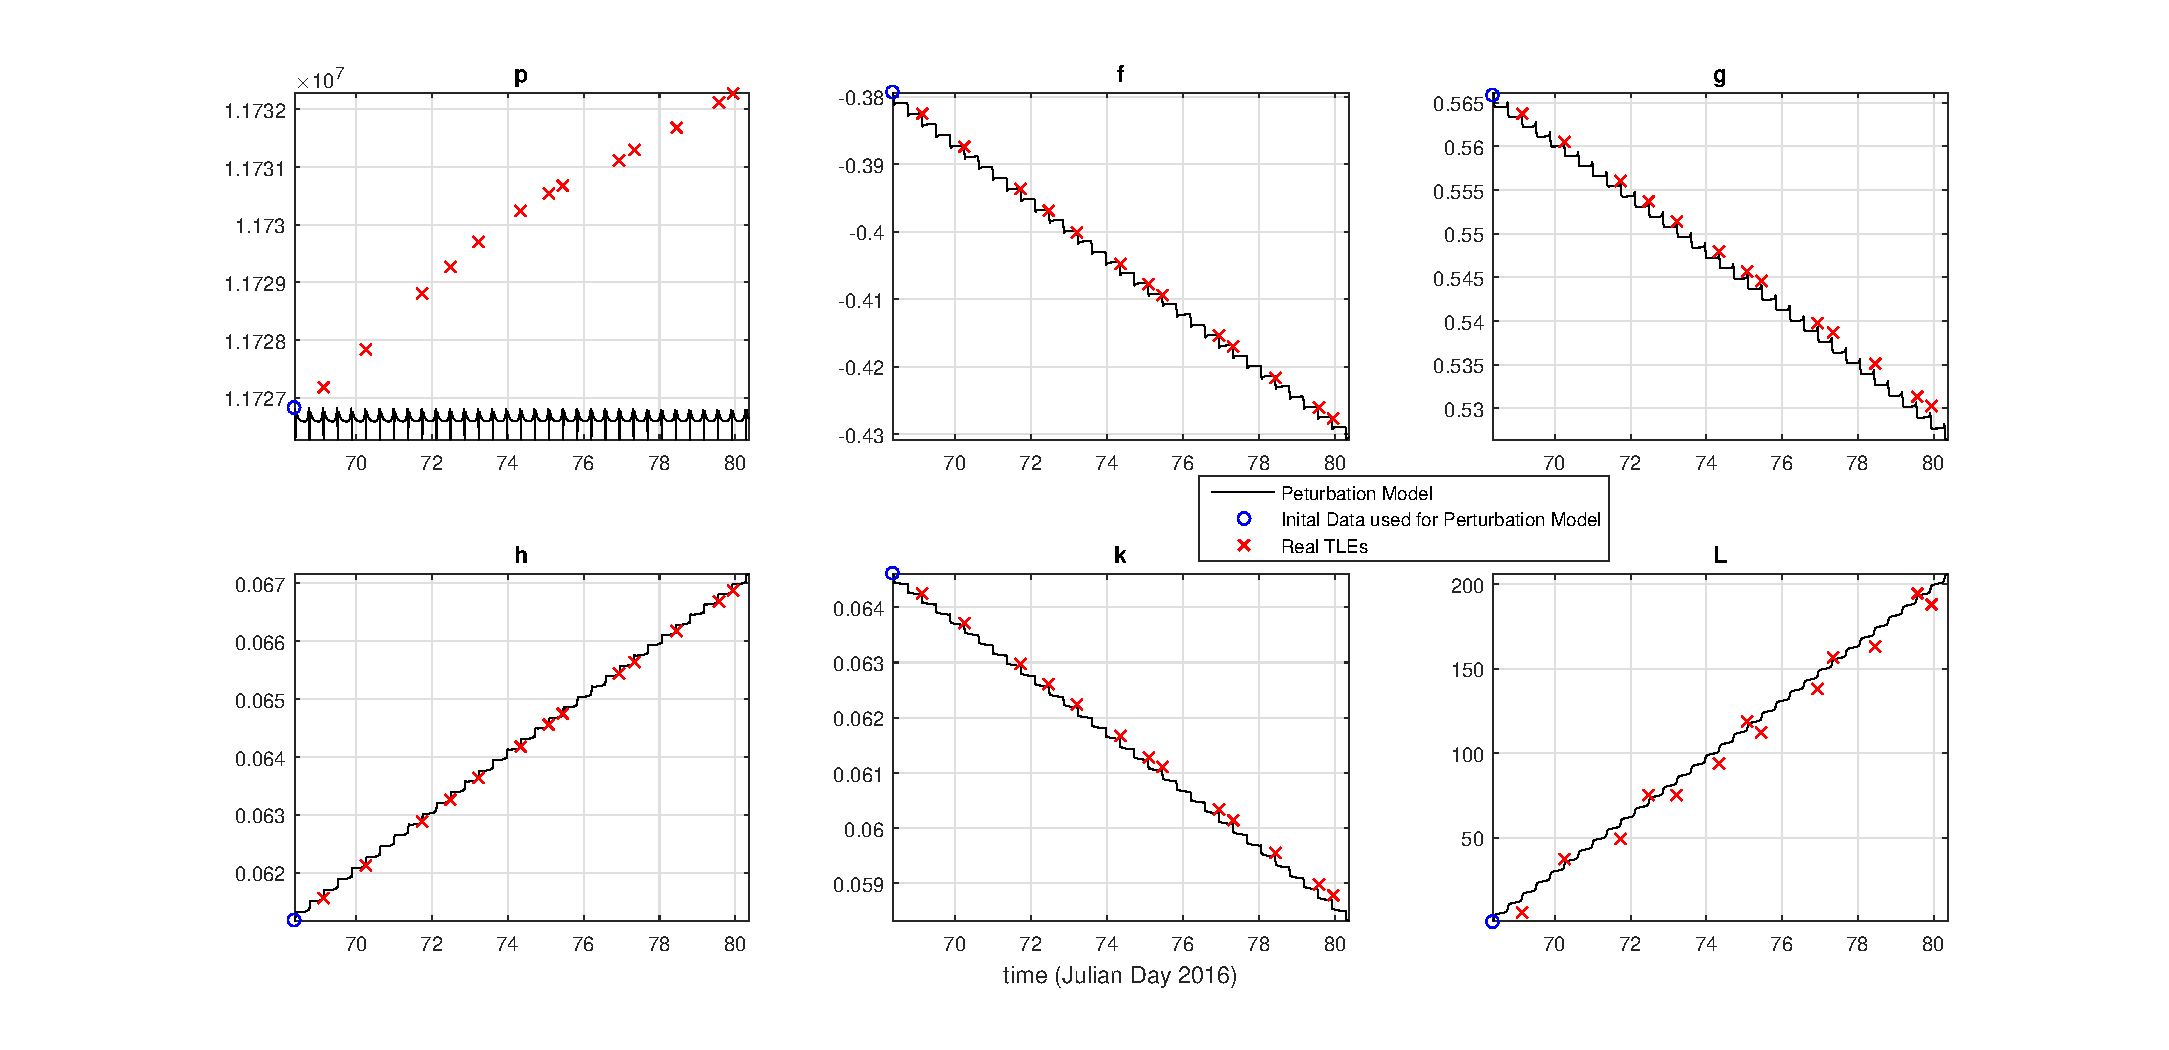
\includegraphics[trim = {3cm 0 3cm 0},clip,width=1\linewidth]{Q2equinoctial_overtime.eps}
\end{figure}



\end{document}